%-----------------------Homework------------------------------------
%-------------------Arman Shokrollahi---------------------------------
%---------------------Coding Theory-------------------------------

\documentclass[a4 paper]{article}
% Set target color model to RGB
\input{preamble.tex}

\begin{document}
\homework{Práctia \#2}{Feb. 25 al 26 de 2019}{MSc. Fausto M. Lagos S.}{}{Aquí va su nombre}{}

En esta práctica se desarrollarán siete planteamientos cada uno con una valoración de un punto. El objetivo de estas práctica es afianzar sus conocimientos antes de la Prueba de Evaluación Continua correspondiente, puede utilizar todo el material bibliográfico a su disposición y también preguntar todo lo que considere necesario. Preste atención al margen derecho donde encontrará premios y bonificaciones adicionales.

\vspace{5mm}

\problem{1} Determine \textbf{analíticamente} el dominio, rango, paridad y sentido de crecimiento de 
\[
  f(x) = \frac{2 - \sqrt{x}}{5x}.
\]
Utilice la graficadora para verificar su análisis.

\vskip 3mm
\solution{}
\vspace{30mm}

\begin{paracol}{2}
\problem{2} La figura siguiente corresponde a la representación geométrica de la función 
\[
  g(x) = x^3 - x
\]
\begin{figure}[ht]
    \centering
    \begin{tikzpicture}[scale = .75]
        \tkzInit[xmin = -3, xmax = 3, ymin = -3, ymax = 3]
        \tkzAxeXY[label options = {font = {\tiny}}]
        \tkzFct[color = myBlue, line width = 1.125pt]{x ** 3 - x}
    \end{tikzpicture}
\end{figure}
\switchcolumn
\begin{itemize}
    \item[a)] Sin resolverlo algebraicamente responda ¿$g(x)$ es una función impar?. Explique.
    \item[b)] Sin utilizar la graficadora. Sobre la gráfica de $g$ dibuje el lugar geométrico de $|g(x)|$.
    \item[c)] ¿Cuál es la paridad de $|g(x)|$? Explique.
    \item[d)] Especule al respecto de si el valor absoluto de toda función impar será siempre una función par.
    \item[e)] Demuestre o refute algebraicamente su especulación en el item d).
\end{itemize}
\end{paracol}
\vskip 3mm
\solution{}
\vspace{30mm}

\problem{3} Analice (determinar Dominio, Rango, Paridad y Sentido de crecimiento) la función dada y construya una aproximación gráfica de su lugar geométrico sin utilizar la graficadora.
\[f(x) =
  \begin{cases}
    x^2 + 2x, & x \leq -1 \\
    x, & -1 < x \leq 1 \\
    -1, & x > 1
  \end{cases}
\]
Verifique con la graficadora que su análisis es correcto.
\vskip 3mm
\solution{}
\vspace{60mm}

\problem{4} Utilice la función 
\[
  f(x) = \frac{1}{x + 1}
\]
para evaluar
\[
  \frac{f(a + h) - f(a)}{h}, \;\;\; h \neq 0.
\]
\vskip 3mm
\solution{}
\vspace{50mm}

\problem{5} \marginnote{\includegraphics[scale = 1]{overleaf}} Sin utilizar la graficadora. Analice la función dada y construya una aproximación gráfica de su lugar geométrico
\[
  f(x) = \sqrt{x^2 - 3x - 10}
\]
\vskip 3mm
\solution{}
\vspace{30mm}

\begin{paracol}{2}
\problem{6} A partir de la gráfica de $f(x)$ dada, determine sus características (Dominio, Rango, Paridad y Sentido de Crecimiento) y de acuerdo a lo que conoce de funciones racionales deduzca la expresión analítica para $f$.
\switchcolumn
\begin{figure}[ht]
    \centering
    \begin{tikzpicture}
        \tkzInit[xmin = -4, xmax = 4, ymin = -6, ymax = 8, ystep = 2]
        \tkzAxeXY[label options = {font = {\tiny}}]
        \tkzFct[color = myBlue, line width = 1.125pt, domain = -4:-1]{(x ** 2 + 1) / (x ** 2 - 1)}
        \tkzFct[color = myBlue, line width = 1.125pt, domain = -1:1]{(x ** 2 + 1) / (x ** 2 - 1)}
        \tkzFct[color = myBlue, line width = 1.125pt, domain = 1:4]{(x ** 2 + 1) / (x ** 2 - 1)}
        \draw[gray!75, dashed] (-1, -3) -- (-1, 4);
        \draw[gray!75, dashed] (1, -3) -- (1, 4);
        \draw[gray!75, dashed] (-4, .5) -- (4, .5);
    \end{tikzpicture}
\end{figure}
\end{paracol}
\vskip 3mm
\solution{}
\vspace{30mm}

\problem{7} La \textbf{función factorial} $f(n) = n!$, cuyo dominio es $\mathbb{Z}$, se define como el producto de los primeros $n$ enteros positivos, i.e. 
\[
  f(n) = n! = 1\cdot 2\cdot 3 \cdots (n - 1) \cdot n.
\]
\begin{itemize}
    \item[a)] Calcule $f(2)$, $f(3)$, $f(5)$ y $f(7)$.
    \item[b)] Muestre que $f(n + 1) = f(n)\cdot(n + 1)$.
    \item[c)] Simplifique $\frac{f(n + 2)}{f(n)}$.
\end{itemize}
\vskip 3mm
\solution{}
\vspace{30mm}

\problem{8} \todo[color = cyan!65!gray]{\small Si resuelve este problema su solución será publicada en la cartelera de matemáticas} In $\triangle ABC$, a point $D$ is on $\overline{AC}$ so that $AB = AD$. $m\angle ABC - m\angle ACB = 30$. Find $m\angle CBD$.
\begin{center}
    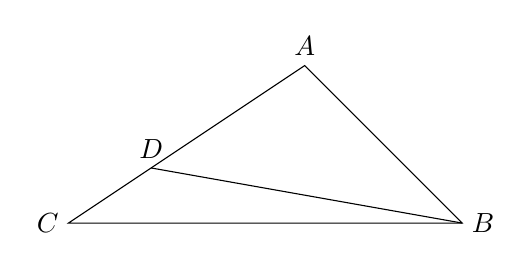
\begin{tikzpicture}
        \coordinate[label = left:{$C$}] (C) at (0, 0);
        \coordinate[label = right:{$B$}] (B) at (5, 0);
        \coordinate[label = above:{$A$}] (A) at (3, 2);
        \coordinate[label = above:{$D$}] (D) at (1.05, .7);
        
        \draw (A) -- (B) -- (C) -- cycle;
        \draw (B) -- (D);
    \end{tikzpicture}
\end{center}
\end{document}
